\documentclass{article}
\usepackage[margin=0.5in]{geometry}
\usepackage{amsmath}
\usepackage{float}
\usepackage{graphicx} % Required for inserting images

\title{Numerical Solution of ODEs using Trapezoidal Rule and Newton-Raphson}
\author{Himanshu Jindal, Shubham Vishwakarma, Kaustubh Dandegaonkar}
\date{}

\begin{document}
\maketitle

\section*{Problem Statement}
Solving System of Differential Equations

Define the vector of dependent variables $\mathbf{Y}$ and the vector of functions $\mathbf{F}(x, \mathbf{Y})$:

\begin{align}
    \mathbf{Y} &= \begin{bmatrix} y_{1} \\ y_{2} \\ y_{3} \end{bmatrix} \\
    \mathbf{F}(x, \mathbf{Y}) &= \begin{bmatrix} f_1(x, \mathbf{Y}) \\ f_2(x, \mathbf{Y}) \\ f_3(x, \mathbf{Y}) \end{bmatrix}
\end{align}


The system of differential equations can be expressed as:

\begin{align}
    \textbf{Y}' &= \mathbf{F}(x, \mathbf{Y})
\end{align}

\section*{Numerical Solution Using Trapezoidal Rule}

To numerically solve this system of differential equations, we employ the Trapezoidal Rule for time discretization. The Trapezoidal Rule is a numerical integration method that can be adapted for solving differential equations.

Let $h$ be the step size and $x_i = x_0 + i \cdot h$. The Trapezoidal Rule updates the solution at each step as follows:

\begin{align}
    \mathbf{Y}^{(i+1)} &= \mathbf{Y}^{(i)} + \frac{h}{2} \left[ \mathbf{F}(x_i, \mathbf{Y}^{(i)}) + \mathbf{F}(x_{i+1}, \mathbf{Y}^{(i+1)}) \right]
\end{align}

Here, $\mathbf{Y}^{(i)}$ represents the solution at the $i$-th step, and $\mathbf{F}(x, \mathbf{Y})$ is the vector function defining the differential equations.

\section*{Theoretical Error Analysis}

The error analysis involves understanding the difference between the numerical solution and the exact solution. Let's consider the local truncation error and the global error.

\subsection*{Local Truncation Error}

The local truncation error at each time step is the error introduced by a single application of the numerical method. 
$$
T_n = \frac{y(x_{n+1}) - y(x_n)}{h} - \frac{1}{2} [ f(x_n, y_n) + f(x_{n+1}, y_{n+1}))
$$
For the Trapezoidal Rule, the local truncation error is proportional to the third derivative of the solution and the square of the step size $h$. The local truncation error for each component of the vector $\mathbf{Y}$ can be expressed as:

\begin{align}
    \text{T}_1 &= \frac{h^2}{12} y_{1}'''(t) + \mathcal{O}(h^3), \\
    \text{T}_2 &= \frac{h^2}{12} y_{2}'''(t) + \mathcal{O}(h^3), \\
    \text{T}_3 &= \frac{h^2}{12} y_{3}'''(t) + \mathcal{O}(h^3).
\end{align}

Here, $\text{T}_1, \text{T}_2,$ and $\text{T}_3$ represent the local truncation error for $y_{1}, y_{2},$ and $y_{3}$, respectively.

\subsection*{Global Error}

The global error is the cumulative error over the entire solution interval. It is influenced by the local truncation error at each step and the total number of steps taken. The global error is typically proportional to the step size $h$ and is given by:

\begin{align}
    \text{Global Error} &= \mathcal{O}(h^2).
\end{align}

This indicates that by reducing the step size, the global error can be effectively decreased.

\section*{Newton-Raphson Method for Iterative Solution}

The numerical solution using the Trapezoidal Rule is implicit and requires an iterative solution. We utilize the Newton-Raphson method for solving the nonlinear equation:

\begin{align}
    \mathbf{F}(\mathbf{Y}_{n+1}) &= \mathbf{Y}_{n} + \frac{h}{2}[\mathbf{F}(x_{n}, \mathbf{Y}_{n}) + \mathbf{F}(x_{n+1}, \mathbf{Y}_{n+1})] - \mathbf{Y}_{n+1}
\end{align}

The Newton-Raphson iteration is employed to find $\mathbf{Y}_{n+1}$ such that $\mathbf{F}(\mathbf{Y}_{n+1}) = \mathbf{0}$. The iterative process is governed by:

\begin{align}
    \mathbf{Y}_{k+1} &= \mathbf{Y}_{k} - [\mathbf{J_F}(\mathbf{Y}_{k})]^{-1} \mathbf{F}(\mathbf{Y}_{k})
\end{align}

where $\mathbf{J_F}(\mathbf{Y}_{k})$ is the Jacobian matrix of $\mathbf{F}$ evaluated at $\mathbf{Y}_{k}$.


\section*{Problem Statement 1}
Solving System of Differential Equations:

\begin{align*}
    y_1' &= -2y_1 + y_2 - 2y_3\\
    y_2' &= y_1 - 2y_2 + 2y_3 \\
    y_3' &= 3y_1 - 3y_2 + 5y_3
\end{align*}

Initial conditions:
\begin{align*}
    y_1(0) &= -2 \\
    y_2(0) &= 2 \\
    y_3(0) &= 4
\end{align*}
\subsection*{Explanation of the Code and Graphs}

The provided Python code implements the numerical solution of the given system of differential equations using the Trapezoidal Rule and the Newton-Raphson method. The functions defined in the code correspond to the system of differential equations, and the main solver uses newton raphson for implicit calculations.

The graphs below depict the numerical solutions (solid lines) obtained by the Trapezoidal Rule and Newton-Raphson method. The exact solutions (dashed lines) are also plotted for comparison. The solutions are calculated over the interval $[0, 1]$ with a step size of $0.0001$.
\begin{figure}[H]
    \centering
    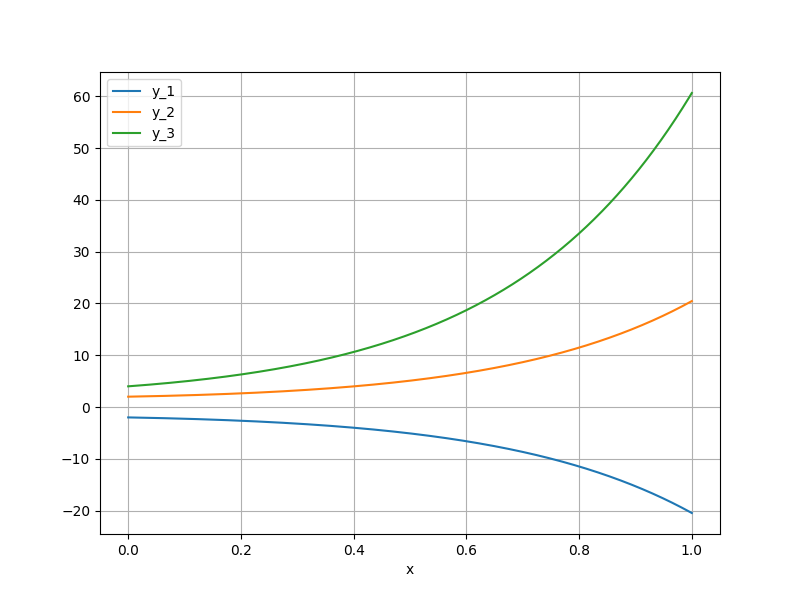
\includegraphics[width = 13cm]{save.png}
    \caption{Caption}
    \label{fig:solutions}
\end{figure}
The figure \ref{fig:solutions} illustrates the accuracy of the numerical method by comparing the computed solutions with the exact solutions. The code provides insights into the implementation of numerical methods for solving differential equations.

\section*{Problem Statement 2}
Consider an electrical circuit consisting of an inductor (L), a resistor (R), and a capacitor (C) described by the following second-order linear differential equation:

\[
L\frac{d^2Q}{dt^2} + R\frac{dQ}{dt} + \frac{1}{C}Q = V(t)
\]

where:
\begin{itemize}
  \item \( Q(t) \) is the charge in the circuit at time \( t \),
  \item \( L = 1 \, \text{H} \) is the inductance,
  \item \( R = 40 \, \Omega \) is the resistance,
  \item \( C = \frac{1}{4000} \, \text{F} \) is the capacitance,
  \item \( V(t) = 24 \, \text{V} \) is the applied voltage.
\end{itemize}

The initial conditions are \( Q(0) = 0 \) and \( \frac{dQ}{dt}(0) = 0 \).

This is similar to Solving System of Differential Equations:

\begin{align*}
    \frac{dI}{dt} &= -40I - 4000Q + 24 \\
    \frac{dQ}{dt} &= I
\end{align*}

Initial conditions:
\begin{align*}
    Q(0) &= Q_0 = 0 \\
    I(0) &= I_0 = 0
\end{align*}
\subsection*{Graphs obtained by the Trapezoid Rule}
h = $5 \times 10^{-5}$
\begin{figure}[H]
    \centering
    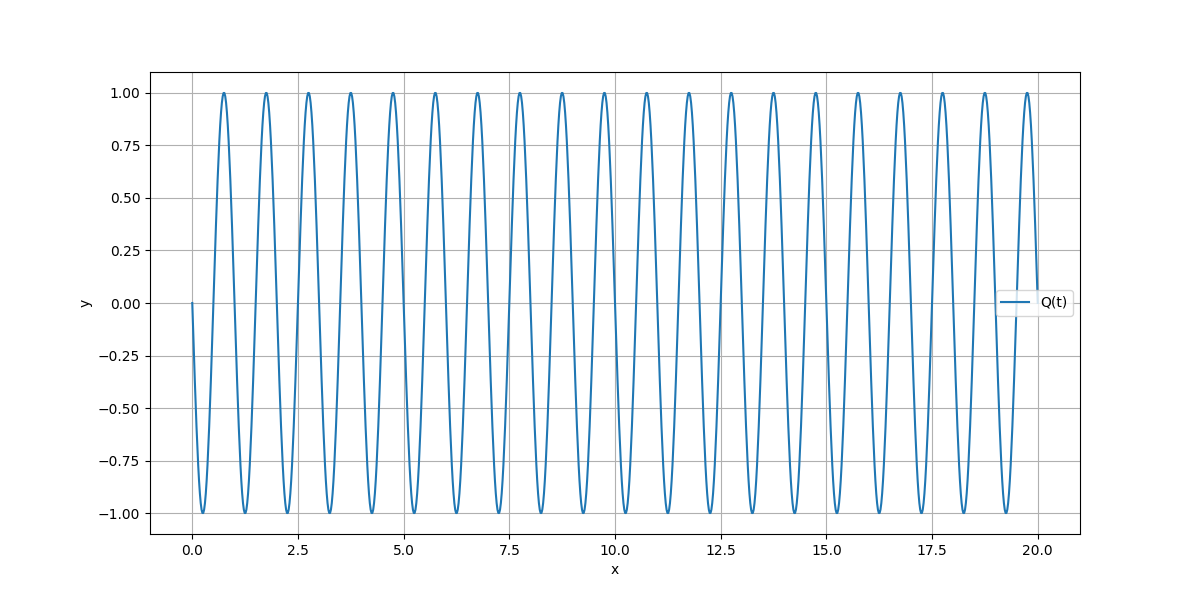
\includegraphics[width = 13cm]{save_0.png}
    \caption{Charge}
    \label{fig:Charge}
\end{figure}

\begin{figure}[H]
    \centering
    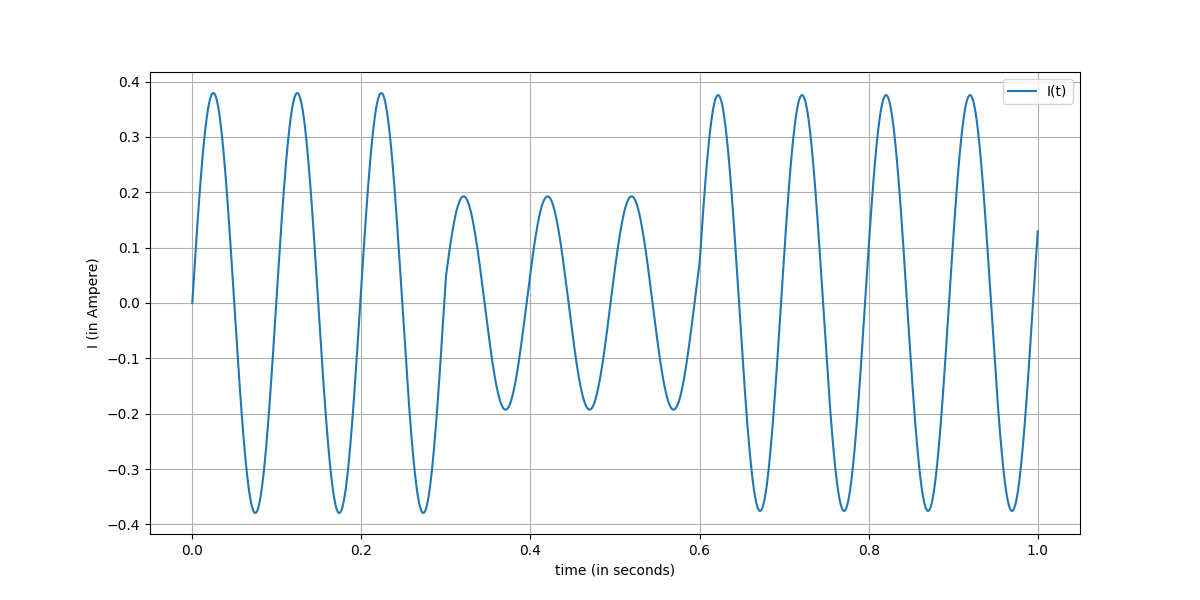
\includegraphics[width = 13cm]{save_1.png}
    \caption{Current}
    \label{fig:Current}
\end{figure}

\subsection*{Actual Graphs}

\begin{figure}[H]
    \centering
    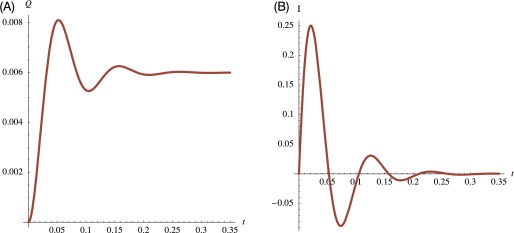
\includegraphics[width = 13cm]{Expected.jpg}      
    \caption{Actual Graphs}
    \label{fig:Actual Graphs}
\end{figure}
\end{document}